\chapter{Applications and Use Cases}
\label{chapter:applications}
\epiquote{If your only tool is a hammer then every problem looks like a nail.}{Abraham Maslow, 1966}

A fascinating aspect of computer science and information technology is, that it has applications in every conceivable domain. It is this combination of purely technological aspects -- the computational part -- and the domain knowledge, that make the field challenging as well as interesting. Digital transformation -- the act of improving businesses and processing using digital technology \cite{Vial:2019Understanding} -- has been a driving force behind economic activity over the past decades, and while many non-technological factors define digital transformation, optimisation through the application of dispruptive technologies remains the main incentive behind it.

Consequently, we do not want to detach the work presented in this thesis from its concrete applications and instead aim to motivate it based on real-world scenarios. In the sections that follow, we will therefore be introducing three use cases, for which we believe that a general-purpose multimedia database system would fulfill an important function. From these use cases, we then go on to derive a series of requirements for such a multimedia database.

\section{Use case 1: Interactive Multimedia Retrieval}
\label{section:application_retrieval}

Multimedia retrieval in a broader sense describes the act of finding items of interest in large multimedia collections, wherein ``multimedia'' can refer to any type of modality, such as text, images, videos or audio and any combination thereof. Consequently, a multimedia retrieval system must be able to have a user express their \emph{information need}, which is translated to a \emph{query} that the system can use to produce the item(s) of interest as a \emph{result}. The process is visualized in \Cref{figure:mr-ideal} and a formal problem definition will be provided in \Cref{chapter:theory_multimedia_analysis_and_retrieval}.

\begin{figure}[tb]
    \centering
    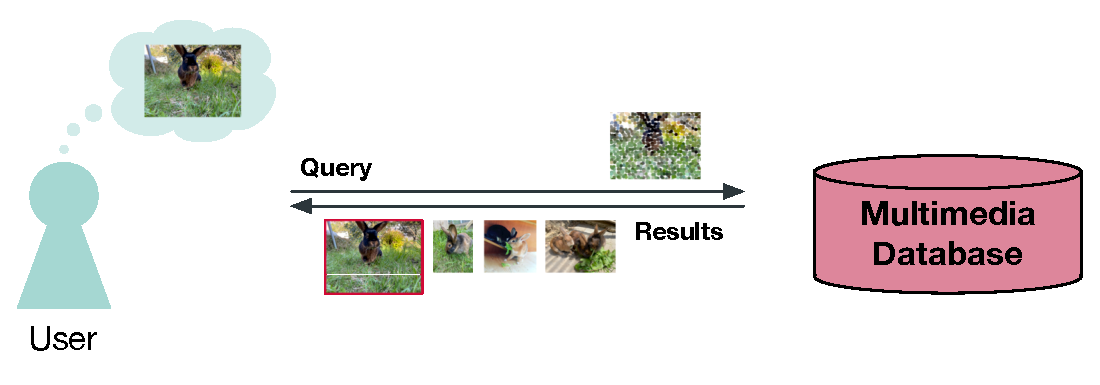
\includegraphics[width=\textwidth]{figures/mr-ideal.eps}
    \caption{The idealised multimedia retrieval problem: A user expresses an information need as a query and the multimedia retrieval system returns matching items from a collection as a result.}
    \label{figure:mr-ideal}
\end{figure}

There are many potential applications of the multimedia retrieval problem, and to name a few examples, one could consider libraries of media items produced by radio or TV stations \cite{Watanabe:1998Multimedia}, collections of cultural heritage data as maintained by museums, archives and archaeology departments \cite{Tsai:2007Review} or medical image databases containing X-rays or \acrshort{mri}s \cite{Mueller:2004Review} that must somehow be made searchable.

What makes multimedia retrieval a challenging problem is the inherently unstructured nature of the data, by which we mean that the raw, (digital) information may not directly reflect the content of the item as a human consumer might perceive or describe it. Let us take, for example, the image of a rabbit the user in \Cref{figure:mr-ideal} is looking for\footnote{On purpose, we do not consider the aspect of reconstructing the image from memory, which makes the problem even more challenging.}. If our task were to describe that image so that we can retrieve it from a large database, we might use terms like ``rabbit'', ``bunny'' or ``grass''. We might assume, judging from the image, that the scene is taking place in a ``garden'' and maybe we notice that the rabbit is currently ``munching'' on a ``leaf'' or ``strain of grass''. We might even know the rabbit's breed or name, if we happened to be its owner.

All of this information is formed based on a series of steps ranging from perception, over interpretation to cognition as illustrated in \Cref{figure:knowledge_formation} and each of these steps is accompanied by a loss or distortion of information \cite{Javanmardi:2021Exploring,Rossetto:2018Multi}, which makes this process highly subjective, giving rise to a series of ``gaps'' that influence the outcome. Most importantly, however, all of the aforementioned descriptions are not explicitly contained in the raw image data, which is merely an array of colour values that constitutes the image and does neither come pre-labeled nor pre-described.

\begin{figure}[tb]
    \centering
    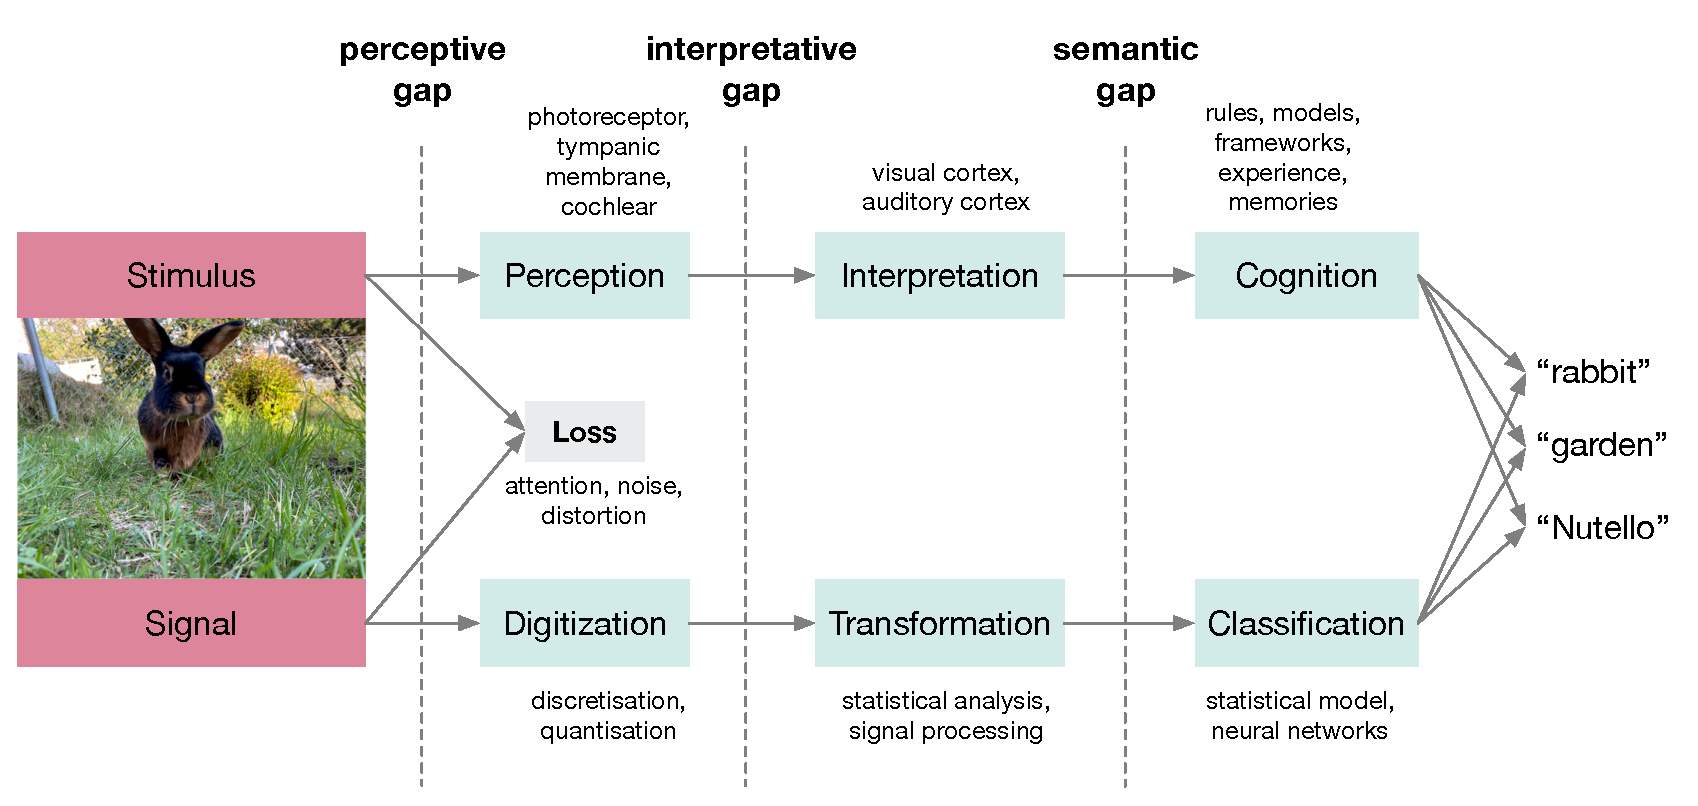
\includegraphics[width=\textwidth]{figures/gaps.eps}
    \caption{A simplified model of knowledge formation from an analogue input in humans (adapted from \cite{Javanmardi:2021Exploring}) and computers.}
    \label{figure:knowledge_formation}
\end{figure}

This impedance mismatch between the content being stored and the information required to find it, is the main challenge that unstructured data brings with it, as opposed to structured data, which consists of retrievable units of information by its very nature. Bridging the gaps between the information available and the information one might use to actually search for an item of interest is therefore one of the obstacles to overcome in multimedia retrieval. Over the years, different solutions have emerged:

\begin{description}
    \item[Manual Labeling] The obvious solution is to manually embed the aforementioned labels and descriptions into the multimedia item so that we can use this information to find it at a later point in time. While as of today, this approach is still widely used, it comes with two important disadvantages. Obviously, it remains a subjective task, because as we have argued, the process of forming these labels may yield different results depending on who is assigning them (due to the perceptive, interpretative and semantic gap). Most importantly, though, the task of manual label assignment is laborious and unable to scale with the large volumes and the ever increasing velocity at which multimedia data is produced. This is related to the general challenge of working with Big Data \cite{Khan:2014Seven}.
    \item[Automatic Labeling] Recent advances in machine learning have provided us with the ability to automatically label \cite{Redmon:2016You} and describe \cite{Radford:2021Learning} different types of multimedia through classification. So instead of annotating the content ourselves, we can leave this to pre-trained models that have, at a high level, a similar mode of operation as a human operator would have, as is illustrated in \Cref{figure:knowledge_formation}. While this solves the problem of scalability, it still remains a subjective task since the process of model training is also prone to the aforementioned gaps found in the data being trained, which can lead to biases \cite{Baer2017:Controlling}. Furthermore, there may be discrepancies between the (mental) model used for classification and the one employed during query formulation, which are typically caried out at different times by different people.
    \item[Content-Based Search] The last approach and the one that ``classical'' multimedia retrieval has concerned itself with for decades is that of \emph{content-based search}. Instead of using the higher-level concepts in the form of textual labels, content-based search works with intermediate representations called \emph{descriptors} that are derived from the data directly using signal processing or statistical analysis. These descriptors -- which are often real-valued vectors \cite{Zezula:2006Similarity} -- can then be used to establish a notion of \emph{similarity} between items in a collection and a query. Instead of a list of exact matches, this type of query returns a ranked list of items that match the query well enough. This is called similarity search \cite{Blanken:2007multimedia} and in this context, the query may refer to more than simply textual input. Given the example in \Cref{figure:mr-ideal}, one could use another image of a rabbit (Query-by-Example, \cite{Kelly:1995Query}) or try to create a sketch (Query-by-Sketch, \cite{Sciascio:1999Content}). One could even come-up with more sophisticated types of queries, such as, searching for poses held by people in an image or video \cite{Heller:2022Multi} or using visual-text co-embeddings \cite{Radford:2021Learning,Spiess:2022Multi} to map textual descriptions to images and vice-versa.
\end{description}

Research has shown that while individual methods falling into any of the three categories may yield acceptable or even exceptional results, there is clear indication that ultimately, a combination of the three is the most powerful solution, especially, since the exact type of information need cannot always be anticipated \cite{Rossetto:2020Interactive}. Furthermore, and partly because different techniques may perform better or worse depending on the information need, we often find that instead of the simple ``issue a query, get a result'' scheme illustrated in \Cref{figure:mr-ideal}, actual multimedia retrieval applications are more interactive and require a back and forth between system and user \cite{Lokovc:2022Task} that involves query (re-)formulation potentially using different descriptors, exploration, examination, query refinement and relevance feedback \cite{Lokovc:2019Interactive,Gurrin:2019Invited} as illustrated in \Cref{figure:mr-actual}. These types of interactive multimedia retrieval systems are explicitly tested at evaluation campaigns such as the \acrfull{vbs} \cite{Schoeffmann:2019Video} or the \acrfull{lsc} \cite{Gurrin:2021Introduction}.

\begin{figure}[tb]
    \centering
    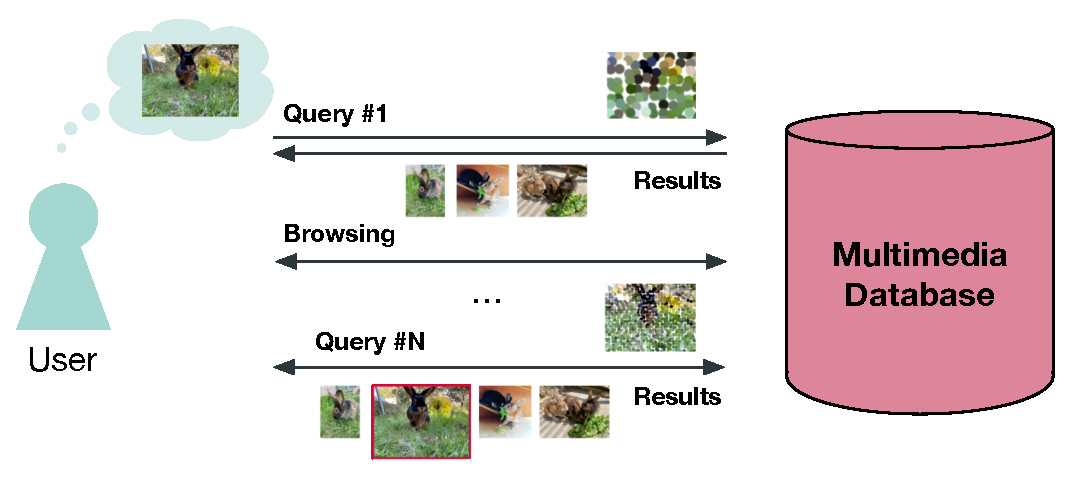
\includegraphics[width=\textwidth]{figures/mr-actual.eps}
    \caption{The interactive multimedia retrieval problem: A continuous back and forth between system and user involving different types of workload as the user tries to find the item of interest through query (re-)formulation, browsing and examination.}
    \label{figure:mr-actual}
\end{figure}
 
Both aspects have important implications for the aforementioned data management system that must support (interactive) multimedia retrieval:

Firstly, such a system must consider different data- and query models when dealing with information from the aforementioned categories as well as a wide range of query workloads. While searching for labels and textual descriptions at scale can be achieved by the well-established \emph{Boolean retrieval} model, we require the completely different \emph{vector space retrieval} model when dealing with descriptors derived from multimedia data and, ideally, we should have the ability to combine the two \cite{Heller:2020Multi}. This is a problem that has been acknowledged by other authors before \cite{Jonson:2016Ten} and that has been partially addressed, for example, by \cite{Giangreco:2018Database,Giangreco:2016Adam,Wang:2021Milvus}.

Secondly, any database management system supporting interactive multimedia retrieval must be able to satisfy the different types of query workloads in a reasonable amount of time, so that the user in the loop must not wait for results too long. One can even state that retrieval speed is more important than perfect accuracy, especially in timeboxed settings such as \acrshort{vbs} or \acrshort{lsc}, because
\begin{enumerate*}[label=(\roman*)]
    \item the retrieval process itself is inherently inaccurate due to the aforementioned gaps, and
    \item there is a user in the loop who examines the results and makes the final decisions.
\end{enumerate*}

A final aspect to consider is the staticity of the data itself. In multimedia retrieval, we often implicitly assume that data collections remain static while they are being queried but it must be emphasized that for most use cases, this is very likely not to be the case. 

\section{Use case 2: Analysis of Social Media Streams}
\label{section:application_online_analysis}

Social media platforms such as Twitter, Facebook, Instagram and TikTok have gained enormous traction over that past few decades. Current estimates suggest, that there are roughly $4.66$ billion active Internet users worldwide, of which $4.2$ billion can be considered active social media users\footnote{Source: Statista.com, ``Social media usage worldwide'', January 2021}. Obviously, this is an enormous market that can be used to place advertisement, reach customers or potential electors and to observe consumer reaction to products and services.

Consequently, social media constitutes an important communcation channel for companies and politicians \cite{Barbera:2018New}. The field of social media analytics aims ``to derive actionable information from social media'' \cite{Zheng:2010Social} (p. 15) for economic, political or scientific purposes. Probably one of the most prominent research challenges involves the identification and countering of ``fake news'' \cite{Lazer:2018Science}, by which we mean information that comes disguised as authentic but contains fabricated, misleading or even wrong information. The term became highly polarised in the 2016 U.S. elections \cite{Quandt:2019Fake} -- when orchestrated campaigns on social media were targeted at voters and may have tipped the scales -- and it has remained a topic high-up on the agenda ever since \cite{Ferrara:2020Characterizing}.

While the problem of fake news can arguably not be solved by mere technological means, the issue has brought about many different research questions in the realm of social media analysis and analytics with potential applications in different domains. One focus lies on the direct detection of misinformation on different channels by different means such as content, propagation patterns \cite{Zhou:2020Survey} or sources. Others try to tackle the detection of bots \cite{Davis:2016BotOrNot,Cresci:2020Decade}, user-accounts that are not backed by real humans and that are often used to create or spread misinformation. And then there is the topic of sentiment analysis \cite{Yue:2019Survey}, which can yield important clues about how (fake-) news stories are received by their consumers.

While many of the aforementioned problems mainly deal with textual information, multimedia obviously plays an important role as well. Instagram and TikTok, for example, focus solely on the sharing of images and videos respectively. A very recent and preliminary analysis suggests \cite{Ciuriak:2022Role}, that the sharing of images and videos plays an important role in the international covering of Russia's war on Ukraine. Potential problems in need of solution could, for example, be the automatic detection of image forgeries \cite{Farid:2009Image} or analysis of the propagation patterns of images \cite{Zannettou:2018Origins}.

If we examine what a fictious and generalised pipleine for social media analysis and analytics would look like, we might arrive at something as illustrated in \Cref{figure:social-media} \cite{Zhu2015:Multimedia,Cui:2019Defend,Yang:2019XFake,Bagade:2020Kauwa}. The many different channels in existence, require a broad range of tools that deal with data collection using crawlers or APIs provided by the respective source. Since all these potential sources are likely to use very different types of data models, some sort of integration into a common framework is very likely. This step may also be accompanied by data enrichtment using external services or data existing in the system's own collection. This is then followed by what we call analysis, which may include a wide range of machine learning and data analysis techniques that may or may not rely on existing data. A common theme for this step is that, similarly to multimedia retrieval, it probably involves generation and storage of formal descriptors of the multimedia content. Therefore, the entire pipeline is very likely to be backed by some type of persistent data store, which contains labels, descriptors and metadata and which allows queries by both the analysis and the analytics components built on top of it. From the described architecture we can, again, derive certain needs with respect to that underlying database: 

\begin{figure}[tb]
    \centering
    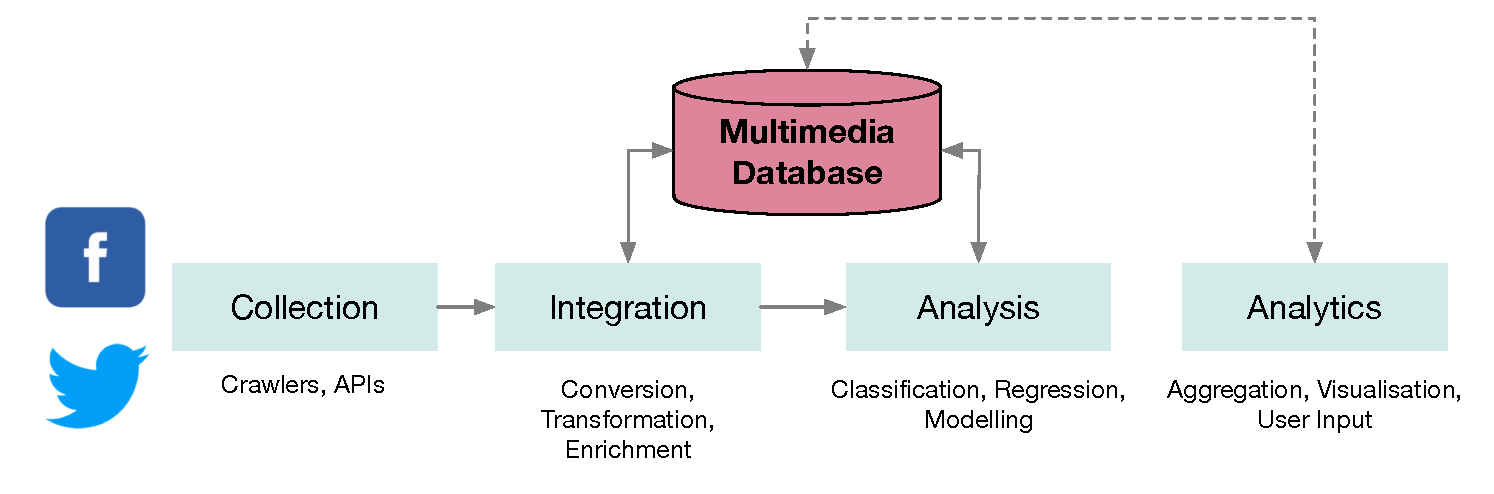
\includegraphics[width=0.90\textwidth]{figures/social-media-architecture.eps}
    \caption{The architecture of a fictious social media analytics platform.}
    \label{figure:social-media}
\end{figure}

Firstly, for this use case, the multimedia database must be able to deal with non-static data, since the various sources potentially generate a steady flow of new information which is likely to be contributing to future inquiries.

Secondly, and similarly to the multimedia retrieval problem, the pipline is likely to deal with structured, semi-structured and unstructured information that must be stored and processed jointly and the multimedia database must be able to cope with this variety. 

And finally, with social media being a very classical field for applying multimedia analytics techniques \cite{Pouyanfar:2018,Jonson:2016Ten}, the different tools built upon the multimedia database are likely to rely on a wide range of query workloads, which the database should be able to accomodate.

\section{Use case 3: Signal Analysis in \texorpdfstring{\acrshort{mrf}}{MRF}}
\label{section:application_mrf}

Multimedia retrieval for medical applications has been an important area of research for many decades now \cite{Mueller:2017Retrieval,Mueller:2004Review} and many of the arguments that we have made in \Cref{section:application_retrieval} can be repeated for this specialised sub-domain.

However, in this section, we focus on a very specific application, in which we do not consider media in the classical sense but in a broader sense of raw signals stemming from a \acrfull{mri} device. One can also refer to this as ``science data'' \cite{Stonebraker:2013SciDB}. \acrshort{mri} is a non-invasive, non-ionizing imaging technique that has gained huge importance in various fields of modern medicine. \acrshort{mri} is enabled by \acrfull{nmr}, which was first described by Purcell and Bloch in 1946 \cite{Bloch:1946Nuclear,Purcell:1946Resonance}. The process behind it is roughly illustrated in \Cref{figure:mri}.

\begin{figure}[b]
    \centering
    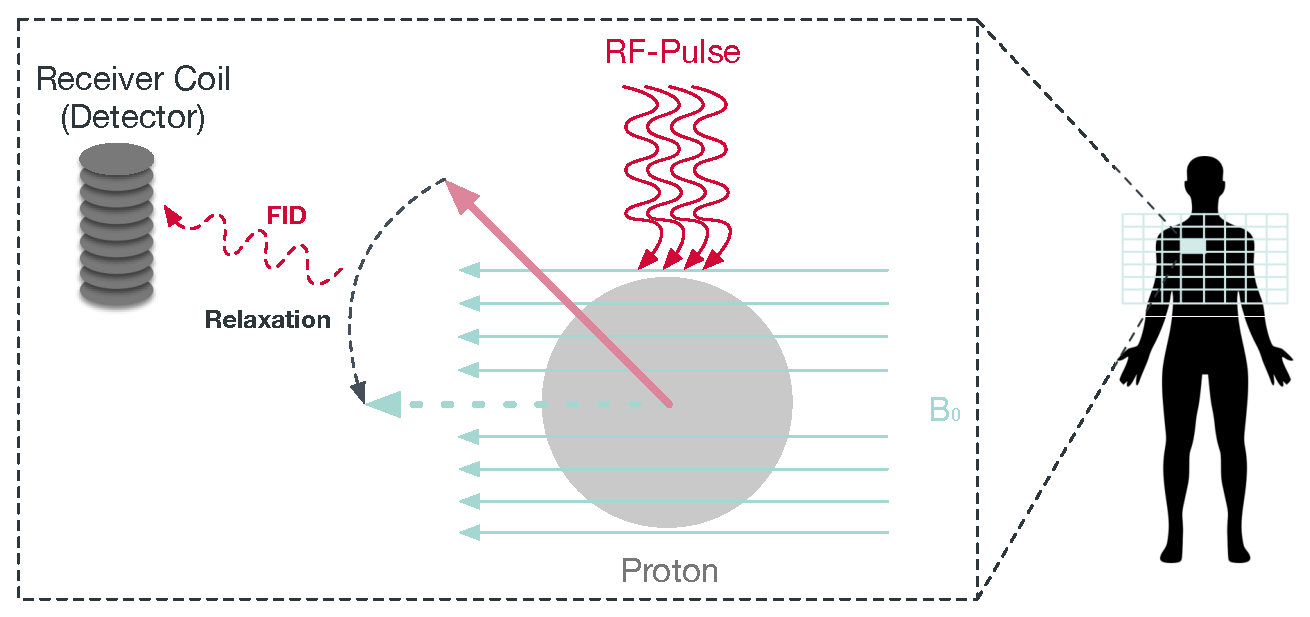
\includegraphics[width=\textwidth]{figures/mri.eps}
    \caption{Simplified illustration of the physical processes enabling \acrshort{mri}.}
    \label{figure:mri}
\end{figure}

In simple terms, an \acrshort{mri}-machine operates by applying a very strong, external, magnetic field - referred to as $B_0$ -- which forces nuclei with a non-zero spin, e.g., a $^{1}\text{H}$ nucleus (proton), to align to and precede around it. That static field is disrupted by applying a second, radio-frequency pulse that interferes with the nucleus' alignment. As this pulse is switched of, the protons start to re-align with $B_0$ over time in what is called relaxation. This process is characterized by the relaxation times $T_1$ (spin-lattice relaxation) and $T_2$ (spin-spin relaxation), which are specific to a type of tissue, and it is accompanied by a measurable, oscillating magnetic field -- the free induction decay --  that induces a current in the detector coil. This signal recorded can be used to reconstruct magnetic properties of the material. To optimise the signal to noise ratio, the procedure is repeated multiple times. Furthermore, spatial resolution is atained by repetition while scanning the body or a specific part thereof. Both aspects contribute to a direct trade-off between acquisition time and image quality.

\acrshort{mri} has the ability to generate fine-grained contrasts in different types of soft tissue. However, it comes with two critical disadvantages: Firstly, there is an inherently long acquisition time that can range anything from several minutes to over an hour per scan, especially when one tries to achieve quantification of magnetic properties of soft tissue. This is an issue because the patient is required to lie still for that time, which they are often unwilling or unable to do. Secondly, and due to this lack of fast, quantitative tools, MRI images have become mostly qualitative in nature. Anatomical areas are often referred to as either ``hyperintense'' or ``hypointense'' with respect to their immediate surrounding, but the difference between such areas or even the absolute values themselves are not measured directly.

\acrfull{mrf} is a technique \cite{Ma:2013Magnetic} that offers a solution to this problem and allows for a quantitative mapping of multiple properties simultaneously while lowering acquisition time. The method is described in \cite{Bipin:2019Magnetic} and illustrated in \Cref{figure:mrf}. In summary, \acrshort{mrf} is based on the assumption that different types of tissue produce a distinct signal evolution -- called \emph{fingerprint} -- when exposed a specific acquisition scheme. This means that during data acquisition, measurements take place under varying (pseudo-random), external magnetic field and RF-pulse configurations and signals are recorded for the different configurations resulting in the fingerprint. That fingerprint can then be matched against a database (called dictionary) of pre-calculated, discretised fingerprints that have been simulated using \emph{Bloch}'s theorem of magnetic resonance \cite{Bloch:1946Nuclear}. Through that matching step, values for $B_0$, $T_1$ and $T_2$ (and other parameters) can be obtained and subsequently used to reconstruct an image. Similarly to \acrshort{mri}, spatial resolution in \acrshort{mrf} is attained by scanning and the described process is therefore repeated several times.

\begin{figure}[tb]
    \centering
    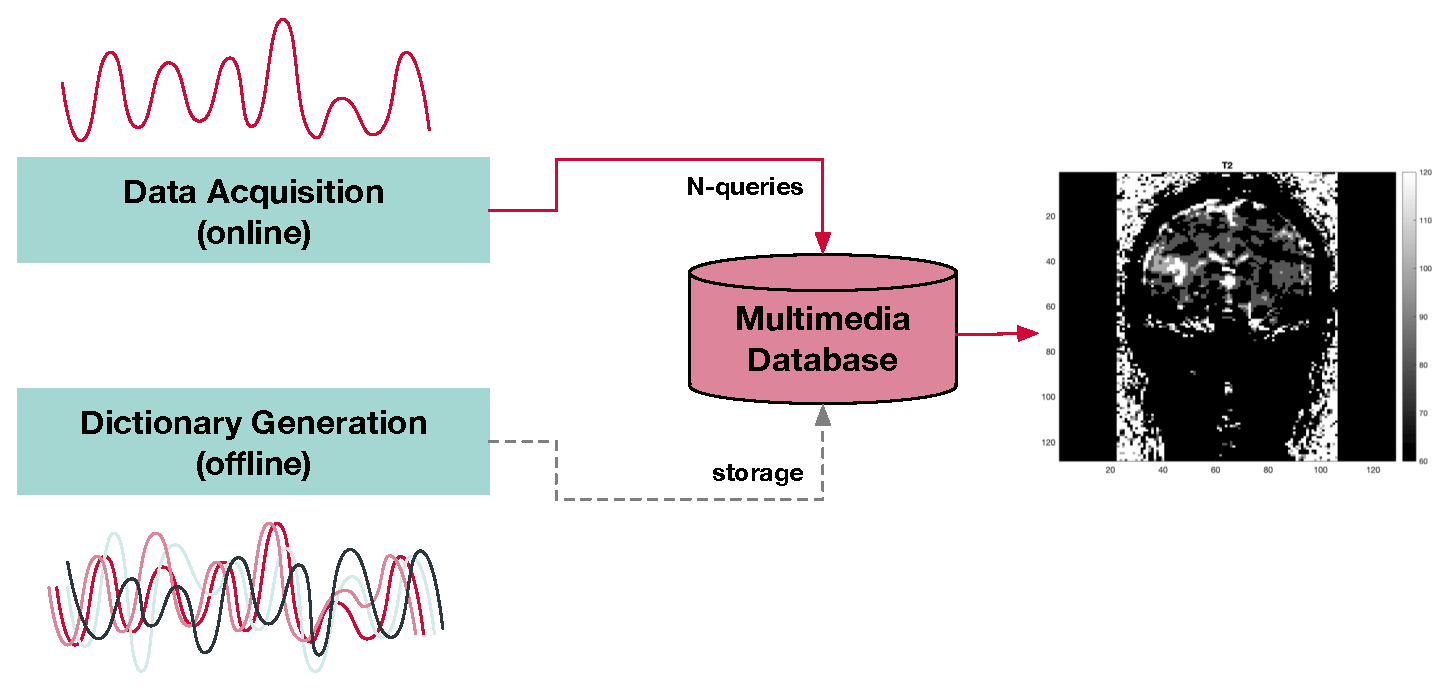
\includegraphics[width=\textwidth]{figures/mrf.eps}
    \caption{Simplified block diagram of a \acrshort{mrf} system (adapted from \cite{Bipin:2019Magnetic}, reconstruction of brain scan kindly provided by Manuel Hürbin).}
    \label{figure:mrf}
\end{figure}

Most \acrshort{mrf} setups implement the pattern matching step as an exhaustive search that retrieves the simulated entry from the dictionary that maximises the inner product with the obtained signal \cite{Bipin:2019Magnetic}. This is called \acrfull{mips} and it involves evaluating the inner product between a complex signal vector and all the vectors in the database. This is a problem related to the similarity search problem being solved in multimedia retrieval, with the difference that the vectors are complex and not real-valued, that the inner product is maximised instead of minimised and that there is interest in a single result per query only. This step constitutes a bottleneck of the entire process, since many queries must be performed in sequence. Several attempts at accelerating it have been made over the years \cite{Mcgivney:2014SVD,Cauley:2015Fast,Cohen:2018MR}.

Once again, we assume that this pattern matching and image reconstruction step should be supported by a dedicated multimedia database, which is a reasonable assumption once dictionaries become so large that they no longer fit into main memory. For a last time, we can try to describe the requirements imposed on such a database: 

Firstly, and similarly to the multimedia retrieval problem, one requires a dedicated data- and query model to store complex vectors and perform \acrshort{mips}. This model differs from the classical, metric-space model applied in multimedia retrieval because it does not restrict itself to real-valued vectors. However, considering complex vectors has been discussed in previous work already, e.g., in the context of similarity search on time series \cite{Rafiei:1997Similarity}. At the same time, the database must also be able to store and access very classical data that fits into the Boolean retrieval model such as the individual parameters $B_0$, $T_1$ or $T_2$. 

Secondly, and also similarly to interactive multimedia retrieval, query time is an important aspect and should be minimised as much as possible, especially in a clinical setup. However, in contrast to multimedia retrieval, this optimisation cannot be bought by trading retrieval quality, because the \acrshort{mrf} problem does not have a human in the loop who might correct an error in an individual query. Instead, the process relies on the lookup of the correct signal vector for every single query. Preliminary work on applying multimedia retrieval techniques to speeding up \acrshort{mrf} pattern matching has shown that sacrificing accuracy leads to sub-optimal image reconstruction results \cite{Huerbin:2020Retrieval,Zihlmann:2021Magnetic} and thus high-dimensional indexing methods known from multimedia retrieval may not be directly applicable.

\section{Deriving Requirements}
\label{section:requirements}
In Sections \ref{section:application_retrieval}, \ref{section:application_online_analysis} and \ref{section:application_mrf} we have discussed three applications that, 
\begin{enumerate*}[label=(\roman*)]
    \item deal with large amounts of unstructured (multimedia) data that must be stored, managed and queried,
    \item use some mathematical descriptors of that unstructured (multimedia) data to enable analysis, comparison and queries,
    \item and that combine these descriptors with data such as labels, descriptions and other information, that must be accessed and sometimes queried as well.
\end{enumerate*}

We acknowledge, that while the details may vary, the basic needs outlined in the aforementioned use cases are overlaping to such an extent that they would benefit from a dedicated multimedia database management system. In fact, the argument for such a system has been made by different authors before us \cite{Adjeroh:1997Multimedia,Smeulders:2000Content,Zahalka:2014towards,Jonson:2016Ten,Khaleel:2021An} and steps towards such a system have been taken \cite{Giangreco:2018Database,Wang:2021Milvus}. However, all concrete approaches somehow narrow the scope in a way that restricts their generalisability.

In this section, we assume that a general-purpose multimedia database is desirable and based on the argument thus far we formalise the requirements imposed on such a system. We do not claim that we address all of the listed requirements in this Thesis. We merely attempt to raise and formalise them, similarly to and based on \cite{Adjeroh:1997Multimedia,Jonson:2016Ten,Khaleel:2021An}.

\subsection{Traditional Database Capabilities}
Regardless of application, any multimedia database is very likely to rely on traditional \acrshort{dbms} capabilities at some point. Be it when data changes or is accessed concurrently and guarantees regarding consistency must be provided or when executing Boolean queries on some aspect of the available metadata. This has been pointed out by \cite{Adjeroh:1997Multimedia,Khaleel:2021An} already and we can therefore reiterate, that a multimedia database must bring the same, basic abilities that any traditional \acrshort{dbms} would w.r.t. to data modeling, data management, execution of Boolean queries and the enforcement of guarantees such as \acrshort{acid} or \acrshort{base}.

\begin{requirement}[label=requirement:classical_dbms]{A Multimedia Database is a \acrshort{dbms}}{}
    At its core, any general-purpose multimedia database is a classical \acrlong{dbms} and should provide the same functionality in terms of data modeling, data management, query execution and guarantees with regards to integrity- and concurrency control, persistence and recovery.
\end{requirement}

\subsection{Multimedia Query Support}
Multimedia queries are fundamentally different in that, as opposed to Boolean queries, they do not produce exact results but instead rely on scores and ranking to quantify similarity between a query and an object in a database. Obviously, a multimedia database system must therefore have the ability to support such queries at all levels from query formulation (i.e., query language) to query execution \cite{Adjeroh:1997Multimedia}. Furthermore, the combination of similarity search with Boolean queries should be possible and well-defined in terms of outcome.

It is worth noting, that by ``Boolean query'' we merely refer to the ability to produce exact matches based on Boolean predicates without making an assumption about the underlying data model. If a multimedia database system choses to implement the graph model then traditional graph traversal queries fall under the category ``Boolean query'' as well.

\begin{requirement}[label=requirement:multimedia_search]{Multimedia Query Support}{}
    A multimedia database must be able to support multimedia queries based on similarity and scores in addition to Boolean queries and it must allow the combination of the two search paradigms in a unified framework.
\end{requirement}

\subsection{Multimedia Data is Big Data}
At its core, dealing with multimedia data equates to dealing with \emph{Big Data} in that a system deals with large \emph{volumes} of information, that may change at a high \emph{velocity} and exhibit a large \emph{variety}, ranging from highly structured metadata attributes to completely unstructured, raw data\footnote{This is known as the ``3 V's of Big Data''. Over time, more of these V's have been described in literature, for example in \cite{Khan:2014Seven}.}. A multimedia database can, of course, favour one of the three aspects over the others (e.g., assume that velocity at which data changes is zero) but in general, all three aspects must be considered jointly, which results in interesting engineering and research problems, e.g., for high-dimensional indexing \cite{Hojsgaard:2019Index} or distribution of data and computation.

\begin{requirement}[label=requirement:big_data]{Multimedia Data is Big Data}{}
    A multimedia database must be able to deal with large volumes of data that exhibit a broad variety and may be subject to change at a high velocity within a single, well-defined framework.
\end{requirement}

\subsection{Modelling Retrieval Quality}

Classical databases produce results that match or don't match a given query, i.e., there is no notion of uncertainty or imprecission in the results. In contrast, the models used in multimedia retrieval are inherently inaccurate to some extent, in that the ``best matching'' entries are obtained, meaning that even bad results may be produced in the absence of better options. This imprecission or inaccuracy is influenced by many factors, not the least of which are the design and choice of the multimedia descriptors themselves.

While the inherent (in-)accuracy of any given descriptor is impossible to predict and thus out of scope for the database that holds it, the notion of accuracy still opens a relevant avenue, since some of that accuracy can be deliberately sacrificed in order to gain speed, which is often done in high-dimensional indexing. Since some use cases are very robust to such decisions while others are not, this aspect must be made explicit at a system level.

\begin{requirement}[label=requirement:quality_model]{Model for Retrieval Quality}{}
    A multimedia database must employ an internal model of quality of results. That model must
    \begin{enumerate*}[label=(\roman*)]
        \item enable a user to specify the desired quality of the result
        \item allow the database system to derive the expected quality for a query execution path
        \item take both aspects into account when planning query execution.
    \end{enumerate*}
\end{requirement}

\subsection{Complex Data Types as First-class Citizen}
Since multimedia analysis and analytics workloads rely on mathematical objects such as vectors, complex numbers or matrices, we argue, that the data model of a multimedia database must be extended to consider those types of data as \emph{first-class citizens} in addition to well-established data types such as numbers or strings. This means, that the structure as well as the mathematical properties of those types must be considered for storage, query planning and execution.

This is not a new idea, per-se, and to some extent self-evident since new use cases obiously require additions to existing data models. Therefore, unsurprisingly, the idea of extensible data models and type systems was already discussed as early as 1988 \cite{Linnemann:1988Design} and it was also argued by \cite{Giangreco:2018Database} that to support multimedia retrieval workloads in a relational database, one must extend the relational model to support those vectors as basic data types. However, it has been pointed out by Michael Stonebraker that the mere ability to model the data, e.g., in the scope of the relational model, is not enough to provide satisfactory performance \cite{Stonebraker:2013SciDB}. He states that ``In summary, RDBMSs seem inappropriate for the vast majority of science applications because they have the wrong data model, the wrong query language, lack important features, and don't provide scalability in an open source code base.'' \cite{Stonebraker:2013SciDB} (p. 56). Similarly, \cite{Whang:2010Tightly} demonstrated that the mere ability to extend a type system with user-defined types through -- what they call -- loose-coupling, is not enough to attain satisfactory performance for queries involving spatial data. The same observation was made when adding information retrieval support \cite{Whang:2015DB} and we add, that this argument can be extended to the handling of multimedia data and associated data types, which are potentially even more complex.

\begin{requirement}[label=requirement:complex_data_types]{Complex Data Types as First-class Citizen}{}
    A multimedia database must treat composite data types (e.g., vectors, complex numbers, matrices, tensors) as first-class citizens of the data, storage and execution model in addition to primitive types such as numbers or strings.
\end{requirement}

\subsection{Functions as First-class Citizen}

All applications considered so far involve the execution of functions that operate on complex data atoms, e.g., to obtain the similarity between a query and items in the database. For a multimedia database to be able to operate effectively, those functions must be considered first-class citizens as well, in that the multimedia database must have the ability to reason about them and make decisions regarding their execution. Hence, they should not be regarded as mere blackboxes, as, for example, a \acrshort{udf}. We argue, that similarly to user-defined types, there is a trade-off between loose- and tight integration of such functions into the \acrshort{dbms}.

This has also been layed out in the 2020 \emph{Seattle Report on Database Research}, where the combination of ``relational algebra and linear algebra in a richer query paradigm'' \cite{Abadi:2020Seattle} (p. 52) is listed as a possible research focus.

\begin{requirement}[label=requirement:functions]{Functions as First-class Citizen}{}
    A multimedia database must treat mathematical functions as first-class citizens of the execution model and must have the ability to reason about those functions' properties during query planning and execution.
\end{requirement}

\section{Mapping Requirements to Contribution}

In reference to the contributions listed in \Cref{section:contributions}, we can make the following mapping between those contributions and the requirements listed in \Cref{section:requirements}:

\begin{description}
    \item[Generalised Model for Similarity Search] addresses \Cref{requirement:multimedia_search} on a theoretical level in that it combines the different query paradigms in a consistent yet versatile framework. The proposed model and especially its implementation also address \Cref{requirement:complex_data_types} and \Cref{requirement:functions} to some extent, with one focus lieing on the optimisation of function execution within a query as well as the connection between index structures and the execution of such functions. However, there are stil many aspects to be explored.
    \item[Adaptive Index Management] provides an answer to the velocity aspect of \Cref{requirement:big_data}, because managing indexes in the face of changing data obviously is a consequence of changing data. As we have argued, these changes can take place fast and they take place concurrently to other query operations, which the multimedia database must handle elastically. The proposed solution is a general-purpose approach and can obviously be complemented with more specialised optimisations at an index level.
    \item[Cost Model for Quality] is a direct consequence of \Cref{requirement:big_data} because, as we will demonstrate, responding to changes in the data can lead to the deterioration of indexing quality. Hence, the multimedia database is forced to decide between one over the other. Since some use cases may tolerate such deterioration while other's do not, the contribution also directly addresses \Cref{requirement:quality_model}.
\end{description}